\chapter{Klasser} \label{chap:klasser}
I dette kapitel vil funktioner i programmet blive forklaret.

\section{Klasser}
\subsection*{Personklasse}
\begin{wrapfigure}[9]{R}{0.25\textwidth}
    \label{img:Person}
    \vspace{-20pt}
    \begin{center}
        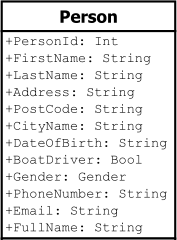
\includegraphics[width=0.2\textwidth]{UmlMini/Person.png}
    \end{center}
    \vspace{-10pt}
    \caption{Person}
\end{wrapfigure}
\textbf{Navn: Person}

\textbf{Felter:}
I personklassen findes felter som indeholder informationer vedrørende personen, såsom navn, alder, adresse, postnr. og kontaktinformation. 
Desuden indeholder klassen også et felt, \textbf{BoatDriver}, som angiver om personen har lov til at føre en båd. \fxnote{Har vi overhovedet anvendt det felt til noget?}

\textbf{Metoder:}
Personklassen indeholder en metode, \textbf{ToString()}, som overrider den eksisterende ToString metode og returnerer personens fulde navn. 
Denne metode er oprette for at gøre det lettere andre steder i programmet at hente personers fulde navne.

\textbf{Anvendelse:}
Personklassen fungerer som baseklasse for SailClubMemberklassen. Grunden til at personklassen og SailClubMember klassen ikke er slået sammen til en klasse er, at personklassen også er grundlag for en gæst i systemet. 
Ved en booking af en sejltur angiver man hvilket hold man skal have med, og i tilfælde af at man skal have en gæst med, som ikke er medlem af klubben, oprettes en instans af personklassen, med de informationer som man angiver i bookingen.

\subsection*{Medlemsklasse}
%Set imagepath and scaling, imagepath set to start in images/ folder, just write filename and extension
\begin{wrapfigure}[6]{R}{0.5\textwidth}
    \label{img:SailClubMember}
    \vspace{-30pt}
    \begin{center}
        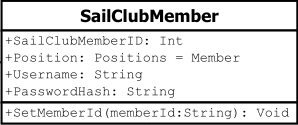
\includegraphics[width=0.48\textwidth]{UmlMini/SailClubMember.png}
    \end{center}
    \vspace{-20pt}
    \caption{SailClubMember}
\end{wrapfigure}
\textbf{Navn: SailClubMember}

\textbf{Felter:}

Basis medlemsklassen for systemet er SailClubMember. 
Klassen er en underklasse til den mere generelle Person klasse. 
Udbyggelsen i denne klasse er, at et medlem har et medlems Id, en position, et brugernavn og et password.

\textbf{SailClubMemberId} bliver brugt i hele systemet til at identificere hvilken bruger der gør hvad. 

\textbf{Positions} feltet angiver at personen er et medlem i klubben. 
Positions feltet kan også sættes til at være administrator, i tilfælde at at personen er administrator. 
Positions feltet angiver desuden hvilke rettigheder de forskellige brugere har, fx har en administrator lov til at tilgå alle funktioner i programmet, mens et medlem ikke har lov til at gå ind i undervisnings delen af programmet. 

\textbf{Username} og \textbf{PasswordHash} felterne anvendes i login systemet, som sikrer at hver bruger kan logge ind på systemet og sikre at de kan tilgå funktionerne.

\textbf{Anvendelse:}

SailClubMember klassen er central i programmet, da alle brugere/medlemmer af sejklubben skal oprettes som et SailClubMember og deri skal deres position i klubben angives, så de kan tilgå de funktioner i programmet som de kunne have gavn af. Derudover findes der i RegularSailTrip-klassen og Logbook-klassen referencer til SailClubMember. Dette gøres så at information om hvem der har foretaget en booking af en båd, og hvem der har skrevet logbogen til den sejltur der blev foretaget. Disse referencer er også vist på det fulde UML-diagram som findes i \myref{UML_diagram}

\subsection*{Elevklasse}

\begin{wrapfigure}[10]{R}{0.5\textwidth}
    \label{img:StudentMember}
    \vspace{-30pt}
    \begin{center}
        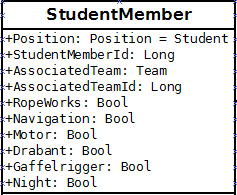
\includegraphics[width=0.48\textwidth]{UmlMini/StudentMember_UML.png}
    \end{center}
    \vspace{-20pt}
    \caption{StudentMember}
\end{wrapfigure}

\textbf{Navn: StudentMember}

\textbf{Felter:}

StudentMemberklassen arver fra SailClubMemberklassen og har derfor alle de felter SailClubMemberklassen også har men StudentMemberklassens \textbf{Position} bliver altid sat til at være 'Student'. \textbf{AssociatedTeam} henviser til det skolehold, den pågældende elev hører til. De seks bool-værdier: \textbf{RopeWorks}, \textbf{Navigation}, \textbf{Motor}, \textbf{Drabant}, \textbf{Gaffelrigger} og \textbf{Night} repræsenterer hver et læringsområde og de bliver sat til 'true' når området er lært. 

\textbf{Anvendelse:}

Denne klasse fungerer som en elev på et skolehold og bruges til at holde styr på ens fremskridt mod at blive bådfører. I løbet af en toårig periode bør man have lært alle områderne og herefter bliver man ``forfremmet'' til SailClubMember og får et bådførerbevis.


\subsection*{Skoleholdklasse}

\begin{wrapfigure}{R}{0.5\textwidth}
    \label{img:Team}
    \begin{center}
        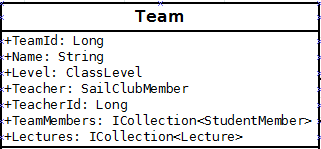
\includegraphics[width=0.48\textwidth]{UmlMini/Team_UML.png}
    \end{center}
    \caption{Team}
\end{wrapfigure}

\textbf{Navn: Team}

\textbf{Felter:}

\textbf{TeamId} bruges til at identificere de enkelte hold fra hinanden. \textbf{Teacher} er den lærer der er tilknyttet holdet og \textbf{Name} er navnet på holdet. \textbf{Level} fortæller om holdet er et første eller andet års hold. Klassen har en ``collection'' (\textbf{TeamMembers}) som der bliver sat \textit{StudentMembers} ind på, hvilket repræsenterer de elever der er på skoleholdet. ``Collectionen'' \textbf{Lectures} indeholder de lektioner som klassen har haft og skal have. \fxnote{Er ikke sikker på dette, det skal omskrives ud fra hvad der bliver skrevet om 'Lecture'-klassen}

\textbf{Anvendelse:}

Teamklassen fungerer som et skolehold. Den bliver brugt til at holde styr på eleverne og bruges som besætningen på en båd, når denne reserveres. 


\fxnote{Er ikke sikker på dette, det skal omskrives ud fra hvad der bliver skrevet om 'Lecture'-klassen}
 
\subsection*{Sejlturs-klasserne}
\begin{wrapfigure}[12]{R}{0.4\textwidth}
    \label{img:SailTrip}
    \vspace{-20pt}
    \begin{center}
        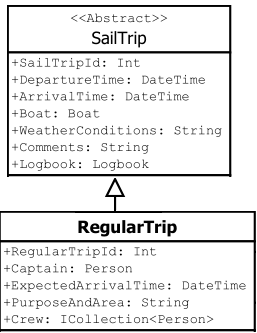
\includegraphics[width=0.35\textwidth]{UmlMini/SailTrip.png}
    \end{center}
    \vspace{-20pt}
    \caption{SailTrip}
\end{wrapfigure}
\textbf{Navn: SailTrip og RegularSailTrip}

I en tidlig designstruktur var det tænkt at programmet skulle have indeholdt flere forskellige typer af sejlture, og derfor blev SailTrip-klassen skabt som værende baseklasse for disse andre klasser. 
Senere blev ideen om at have flere typer sejlture ændret og i stedet blev der valgt at der kun skulle være én sejlturstype. 
SailTrip-klassen er dog bibeholdt i tilfælde af videre udbygning af programmet.
Dog findes der enkelte felter i klasserne som overlapper hinanden lidt, men felter er også bibeholdt i tilfælde af udbygning til flere typer sejlture.

\textbf{Felter:}

SailTrip og RegularSailTrips felter udfyldes med informationer vedrørende en sejltur.
Felterne \textbf{DepartureTime} og \textbf{ArrivalTime} indeholder inforamtioner om hvornår sejlturen starter og hvornår den slutter.

Der findes en refererence til et object af typen \textbf{Boat} i SailTrip.
Denne reference kobler en sejltur sammen med en bestemt båd, således at der holdes styr på hvilke både der er optaget hvilke tidspunkter.

Desuden findes der i begge klaser et Id,\textbf{SailTripId}/\textbf{RegularTripId}, som bruges til at adskille de forskellige sejlture fra hinanden.

I RegularSailTrip findes der desuden en samling af personer i feltet \textbf{Crew}.
Her er det værd at bemærke at besætningen er en samling af typen \textbf{Person}, hvilket gør det muligt at vælge besætningsmedlemmer som ikke er medlemmer af klubben, da de kan oprettes som gæster, og derved tilføjes til besætningen.

I SailTrip er der også en reference til en \textbf{Logbook}.
Når en sejltur oprettes i form af en booking, bliver logbogen sat til at være tom.
Først når turen er omme og vedkommende, som foretog bookingen, logger ind i programmet og udfylder logbogen for turen, vil den indeholde data.

\textbf{Anvendelse:}

SailTrip-klassen anvendes kun som baseklasse for RegularSailTrip-klassen. 
RegularSailTrip er derimod en central del i programmet, da det ene hovedformål for programmet er at gøre det muligt at foretage bookings gennem et program. Det andet hovedformål, undervisningsdelen, gør også brug af sejlturene. \fxnote{nogen der har styr på undervisnings delen må gerne lige skrive ind hvordan sejlturene bliver anvendt der}

\subsection{Eventklasse}

\begin{wrapfigure}[10]{R}{0.5\textwidth}
    \label{img:login_interface}
    \vspace{-20pt}
    \begin{center}
        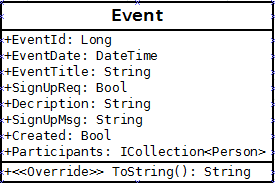
\includegraphics[width=0.48\textwidth]{UmlMini/Event.png}
    \end{center}
    \vspace{-20pt}
    \caption{Eventklasse}
\end{wrapfigure}

\textbf{Navn: Event}

\textbf{Felter:}
Klassen består af 7 felter: \textbf{EventDate}, \textbf{EventTitle}, \textbf{SignUpReq}, \textbf{Description}, \textbf{SignUpMsg}, \textbf{Created} og så en liste af klassen Person, som hedder \textbf{Participants}.

\textbf{Description} er selve begivenhedsbeskrivelsen. 

Den eneste metode er en override af ToString, som retunerer \textbf{Description}.

\textbf{Anvendelse:}

Eventklassen er den klasse om bruges til oprettelse af  begivenheder, nødvendigvis ikke sejlbegivenheder, men generelle begivenheder. Et eksempel kunne være en grillaften eller natsejlads.

\textbf{Participantslisten} bruges når folk skal tilmeldes til begivenhederne; hver begivenhed har sig egen liste med tilmeldte. 

\subsection*{Logbook}
\begin{wrapfigure}[9]{R}{0.25\textwidth}
    \label{img:logbook}
    \vspace{-20pt}
    \begin{center}
        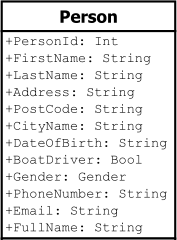
\includegraphics[width=0.2\textwidth]{UmlMini/Person.png}
    \end{center}
    \vspace{-10pt}
    \caption{Logbook}
\end{wrapfigure}
\textbf{Navn: Logbook}

\textbf{Felter:}

\textbf{Metoder:}

\textbf{Anvendelse:}

